\documentclass [titlepage,12pt,letter] {article}
\pagestyle{myheadings}


\usepackage{graphicx} 
\usepackage{epsfig}
\usepackage{subfigure}
\usepackage{fancyhdr}
\usepackage{url} 
\usepackage{amsmath}
\usepackage{algorithm} 
\usepackage{algorithmic}
\pagestyle{fancy}



\fancyhead{}
\fancyfoot{}
			
\lhead{CSC349A Lecture Notes}
\rhead{Little, Rich}


\setcounter{page}{1}
\cfoot{\thepage}




\begin{document} 


These are the lecture notes for CSC349A Numerical Analysis taught by
Rich Little. They roughly correspond to
the material covered in each lecture in the classroom but the actual
classroom presentation might deviate significantly from them depending
on the flow of the course delivery. They are provided as a reference to
the instructor as well as supporting material for students who miss
the lectures. They are simply notes to support the lecture so the text
is not detailed and they are not thoroughly checked. Use at your own
risk. They are complimentary to the handouts. Many thanks to all the
guidance and materials I received from Dale Olesky who has taught this
course for many years and George Tzanetakis. 

\section{Ordinary Differential Equations}

\begin{itemize}
\item{Corresponds to Handouts 34-37 and Chapter 25 in the text.}
\item{We did this way back in Lecture 1 when we solved the parachutist problem analytically and numerically.}
\item{These correspond to solving first-order, initial-value ordinary differential equations.}
\item{That is, solving for $y(x)$ given,
\[
y'(x)=f(x,y(x)) \text{ and } y(x_0) = y_0
\]}
\item{Here, $x$ is the independent variable, $y$ the dependent variable as a function of $x$, and $f(x,y(x))$ is a function of $x$ and $y$.}
\item{The goal is to determine $y(x)$ over $a \leq x \leq b$ given $a=x_0,b,y_0$ and $f(x,y(x))$.}
\end{itemize}

{\bf Example 1: Analytic Method}

Determine $y(x)$ for $0 \leq x \leq 2$ such that
\[
y'(x) = y - x^2 + 1
\]
subject to $y(0) = 0.5$.

\vspace{\baselineskip}
This problem has an analytic solution, namely \[y(x) = (x+1)^2 - 0.5e^x\]. 

Note that I have not showed the analytic solution's steps and I won't expect you to do this either. Our goal is to learn how to approximate the values of $y(x)$ over the given range, not find the function itself.

\subsection{Numerical Methods}

All numerical methods we will consider for approximating $y(x)$ are called {\bf difference methods}:  that is, the continuous, exact solution $y(x)$ is approximated by a \underline{finite set} of computed values at a set of \underline{mesh points} $x_0,x_1,...,x_N$  in $[a,b]$.

For now, we consider only equally-spaced mesh points, and let
\[
x_i=a+ih=x_0+ih, \text{ for } i=0,1,2,...,N
\]
where
\[
h=\frac{b-a}{N}					 
\]
is called the \underline{step size}.

{\bf Notation:} At each of the $N+1$ mesh points $x_i$, the exact solution is denoted by $y(x_i)$ and the approximate solution by $y_i$.

\begin{figure}[h] 
  \centering
  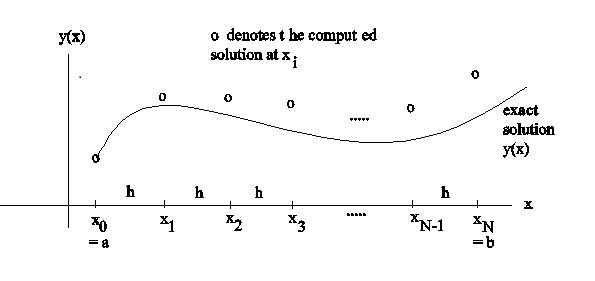
\includegraphics[scale=0.7]{solving_odes}
  \label{fig:solving_odes}
\end{figure}

\section{Euler's Method}

In general, we derive iterative formulas of the form
\[ y_{i+1}=y_i + \phi h \]
where $\phi$ is the slope of the tangent at $x_i$.
\begin{itemize}
\item{Usually, we approximate $\phi$. This is done in different ways for different methods.}
\item{In Euler's Method the right hand side of the differential equation itself gives us an approximation of $\phi$ at each point.}
\item{Recall, $y'(x)=f(x,y(x))$ is the form of the ODEs we are looking at.}
\item{So, at each step $i$ we let $\phi = f(x_i,y(x_i))$.}
\end{itemize}

\subsection{Derivation of Euler's Method}

Taylor's Theorem for $y(x)$ (with $n=1$) expanded about $x_i$ is
\[
y(x)=y(x_i)+hy'(x_i)+\frac{h^2}{2}y''(\xi)
 \]
for some value $\xi$ between $x_i$ and $x$.  Thus, at $x=x_{i+1}$,
\[
y(x_{i+1})=y(x_i)+hy'(x_i)+\frac{h^2}{2}y''(\xi)
\]
where $h=x_{i+1}-x_i$.

For small $h$, this suggests the approximation
\[
y(x_{i+1}) \approx y(x_i)+hy'(x_i)
=y(x_i)+hf(x_i,y(x_i)),
 \]
using the differential equation $y'(x)=f(x,y(x))$. 

Here, we use exact solutions $y(x_i)$ but at each iteration we generally use previous approximations $y_i$. So, Euler's Method approximates each $y(x_{i+1})$ by
\[
y_{i+1}=y_i+hf(x_i,y_i)
\]
for $i=0,1,2,...,N$ where $y_0=y(x_0)$ is the initial condition.

\subsection{Example 2: Euler's Method}

Consider the initial-value problem
\[
y'(x)=y-x^2+1, \text{ subject to } y(0)=0.5.
\]
The first few computed approximations $y_i$ and the corresponding exact solutions $y(x_i)$ are as follows:

\begin{align*}
y_1&=y_0+hf(x_0,y_0) \\
&=0.5+(0.2)(0.5-0^2+1) \\
&=0.5+(0.2)(1.5) \\
&=0.8
\end{align*}
Compared to the exact solution from Example 1 above,
\begin{align*}
y(0.2)&=(0.2+1)^2-0.5e^{0.2} \\
&=1.44-0.5(1.221402758) \\
&=0.829298621
\end{align*}
This gives a true absolute error of,
\[|E_t|=|0.829298621-0.8|=0.0292986\]

The next approximated point can be found as follows,

\begin{align*}
y_2&=y_1+hf(x_1,y_1) \\
&=0.8+(0.2)(0.8-(0.2)^2+1) \\
&=0.8+(0.2)(1.76) \\
&=1.152
\end{align*}
Compared to the exact solution from Example 1 above,
\begin{align*}
y(0.4)&=(0.4+1)^2-0.5e^{0.4} \\
&=1.96-0.7459123488 \\
&=1.2140877
\end{align*}
This gives a true absolute error of,
\[|E_t|=0.0620877\]

The following table summarizes for the first 5 points.

\begin{center}
\begin{tabular}{c|c|c|c}
$x_i$ & $y_i$ & $y(x_i)$ & $|y(x_i)-y_i|$ \\
\hline
0 & 0.5 & 0.5 & 0 \\
0.2 & 0.8 & 0.8292986 & 0.0292986 \\
0.4 & 1.152 & 1.1240877 & 0.0620877 \\
0.6 & 1.5504 & 1.6489406 & 0.0985406 \\
0.8 & 1.98848 & 2.1272295 & 0.1387495
\end{tabular}
\end{center}

Note that the error is actually getting bigger after each step. We will explore this for the rest of the lecture.

\section{Geometric Interpretation of Euler's Method}

$y_0=y(x_0)$ is the intitial condition. Using this value, we compute
\[
y_1=y_0+hf(x_0,y_0)=y_0+hy'(x_0)
\]
from which it follows that
\[
y'(x_0)=\frac{y_1-y_0}{h}=\frac{y_1-y_0}{x_1-x_0}
\]
Geometrically, this says that $y_1$ is obtained from $y_0$ by constructing the tangent line to the graph of $y(x)$ at $x_0$ (which has slope equal to $y'(x_0)$) and going a distance $h$.

\begin{figure}[h] 
  \centering
  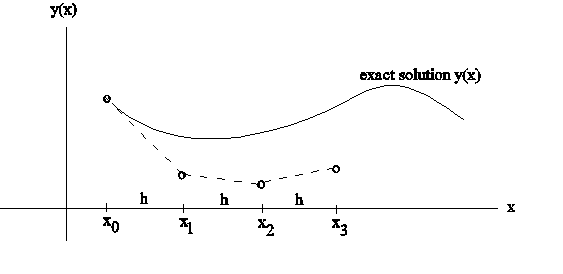
\includegraphics[scale=0.65]{eulers}
  \label{fig:eulers}
\end{figure}

Similarly,
\[
y_2=y_1+hf(x_1,y_1)
\]
so $y_2$ is determined by constructing a straight line through $(x_1,y_1)$ with slope $f(x_1,y_1)$ (not $f(x_1,y(x_1))$, the exact slope).  

{\bf Notes on Euler's Method}

In general, $y_{i+1}$ is obtained by constructing a straight line through $(x_i,y_i)$ with slope equal to $f(x_i,y_i)$, which is an approximation to $y'(x_i)$.

\vspace{\baselineskip}

As $y_i$ depends on $y_{i-1}$, which in turn depends on $y_{i-2}$ and so on, successive values of $y_i$ tend to be less and less accurate (as the truncation errors accumulate as you go across the interval $[a,b]$).

\section{Error Analysis of Euler's Method}

{\bf Truncation Error}

The {\bf total truncation error} in each computed approximation $y_{i+1}$ is composed of two parts:
\begin{enumerate}
\item{the {\bf local truncation error} is the amount of truncation error that results from \underline{a single application} of a numerical method (that is, from the computation of $y_{i+1}$ from $y_i$), and}
\item{the {\bf global truncation error} contains the \underline{accumulated local truncation errors} from all of the steps leading up to the computation of $y_{i+1}$.}
\end{enumerate}

\subsection{Global Truncation Error}

{\bf Definition:} $|y(x_i)-y_i|$ is called the {\bf global truncation error} at $x_i$.

\vspace{\baselineskip}

{\bf Definition:} If the global truncation error is $O(h^k)$, the numerical method used to compute the values $y_i$ is said to be of {\bf order $k$} (or a $k^{th}$ order method).

\vspace{\baselineskip}

{\bf Definition} A numerical method is said to be {\bf convergent} (with respect to the differential equation it approximates) if
\[
\lim_{h\to0} \max_{1 \leq i \leq N} |y(x_i)-y_i|=0
\]

{\bf Notes on Global Truncation Error}

The order of a method is a measure of the accuracy of the computed approximations, or of the rate of convergence of the computed approximations $y_i$ to the exact solutions $y(x_i)$ as $h \rightarrow 0$.

\vspace{\baselineskip}

For any fixed value of the step size $h$, the \underline{larger the order} $k$, the more accurate are the computed approximations.
			 .
\subsection{Derivation of Local Truncation Error for Euler's Method}

{\bf Definition:} The {\bf local truncation error} at any point $x_{i+1}$ is the amount of truncation error that would result from using a numerical method with the exact value $y(x_i)$ rather than the computed approximation $y_i$

\begin{figure}[h] 
  \centering
  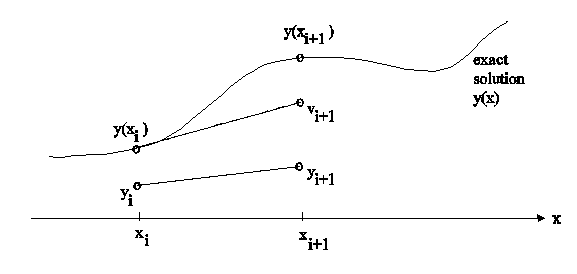
\includegraphics[scale=0.65]{local_trunc}
  \label{fig:local_trunc}
\end{figure}

Recall, Euler’s method is
\[
y_{i+1}=y_i+hf(x_i,y_i).
\]
Using the exact value $y(x_i)$ in this formula instead of the computed approximation $y_i$, define
\begin{equation}
v_{i+1}=y(x_i)+hf(x_i,y(x_i)).
\end{equation}
Then the local truncation error at $x_{i+1}$ is equal to
\[
|y(x_{i+1})-v_{i+1}|.
\]

\subsection{Order of the Local Truncation Error for Euler's Method}

We use Taylor's Theorem,
\[
y(x_{i+1})=y(x_i)+hy'(x_i)+\frac{h^2}{2}y''(\xi_i)
\]
where $h=x_{i+1}-x_i$ and $\xi_i \in [x_i,x_{i+1}]$. So,
\begin{equation}
y(x_{i+1})=y(x_i)+hf(x_i,y(x_i))+\frac{h^2}{2}y''(\xi_i).
\end{equation}
Now, (2)-(1) gives,
\[
|y(x_{i+1})-v_{i+1}|=\left |\frac{h^2}{2}y''(\xi_i) \right |.
\]
Thus, Euler's Method is $O(h^2)$ locally.

\subsection{Example 3: Local Error}

Recall the initial-value problem
\[
y'(x)=y-x^2+1, \text{ subject to } y(0)=0.5.
\]
The first two computed approximations $y_i$ and the corresponding exact solutions $y(x_i)$ are:

\begin{align*}
y_1&=0.8, y(x_1)=y(0.2)=0.829298621, |E_t|=0.0292986 \\
y_2&=1.152, y(x_2)=y(0.4)=1.2140877, |E_t|=0.0620877
\end{align*}

Thus,

\begin{align*}
v_2&=y(x_1)+hf(x_1,y(x_1)) \\
&=0.829298621+(0.2)(0.829298621-(0.2)^2+1) \\
&=0.829298621+0.357859724 \\
&=1.187158345
\end{align*}

Therefore, the local error at point $x_2=0.4$ is $|y(x_2)-v_2|=|1.2140877-1.187158345|=0.026929355$. Note that this value is less than the global error of 0.0620877, given above.

\subsection{Relationship between Local and Global Error for Euler's Method}

An informal justification for the relationship between the local and global truncation errors for Euler's method is as follows:

The local truncation error in each step of Euler's method is, as shown above, $O(h^2)$.

After $N$ steps of Euler's method, the global truncation error $|y(x_N)-y_N|$ of the final computed approximation $y_N$ at $x_N$ will depend on the $N$ local truncation errors of $y_1,y_2,...,y_N$.

But the magnitude of $N$ local truncation errors is 
\[
N \times O(h^2)=\frac{b-a}{h} \times O(h^2) = O(h) \text{ since } h = \frac{b-a}{N}
\]

{\bf Theorem:} (for any method)
If the local truncation error is $O(h^{k+1})$, then the global truncation error is $O(h^k)$. That is, the numerical method used to compute the approximate solution has {\bf order $k$}.  

Thus, the global truncation error for Euler’s method is $O(h)$, and Euler’s method has order 1.

Usually, you cannot compute either the global or local errors exactly. Also, the global error is difficult to approximate directly. But, there are good ways of approximating the local errors which can then be used to approximate the global error. For example, in Euler's method we can use 
\[
E_a=\frac{f'(x_i,y_i)}{2}h^2
\]
as an approximate local truncation error.

{\bf Disadvantages of Euler's Method}
\begin{itemize}
\item{Euler's method is not sufficiently accurate.}
\item{Because the global truncation error is only $O(h)$, a very small step size $h$ is required to compute highly accurate approximations.}
\item{Euler is not often used.}
\item{Methods with a higher order of accuracy are used in practice.}
\end{itemize}

\end{document} 















